% NOTE: paired with figures/01_dgm_comparisons_swe.tex — see the note there
% and paper/supplementary/source-attribution.md.
\begin{figure}[ht]
\centering
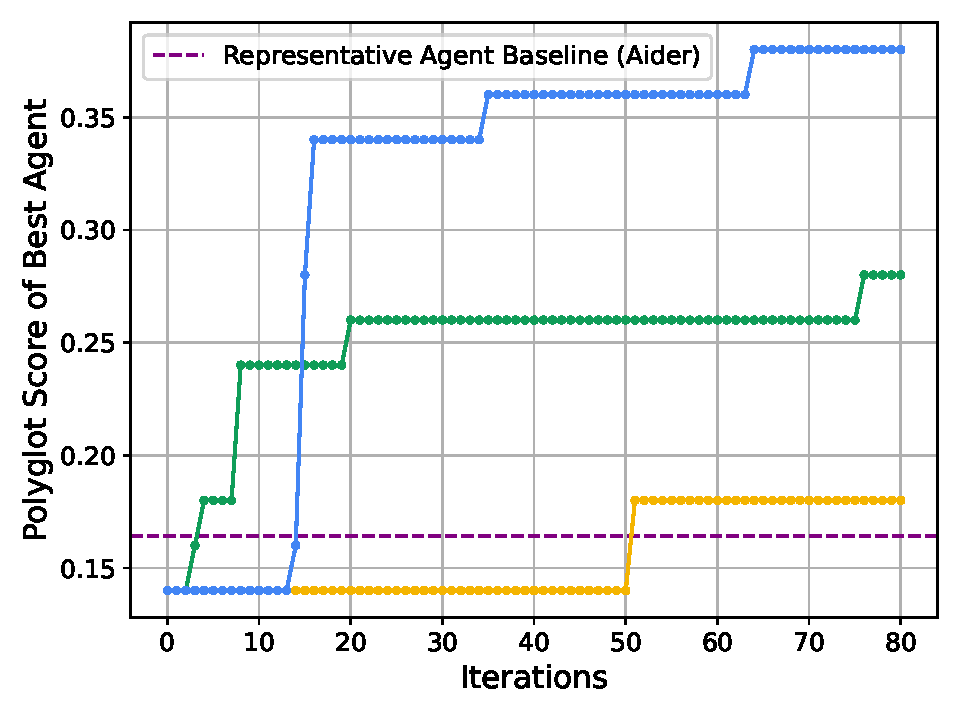
\includegraphics[width=0.7\textwidth]{figures/srcs/02_dgm_comparisons_polyglot.pdf}
\caption{\textbf{Self-improvement and open-ended exploration enable the DGM to continue making progress and improve its performance.} The DGM automatically discovers increasingly better coding agents and performs better on both (Left) SWE-bench and (Right) Polyglot. It outperforms baselines that lack either self-improvement or open-ended exploration, showing that both components are essential for continual self-improvement. These scores are obtained from evaluating on the benchmark subsets detailed in \Cref{sec:benchmarks}. (Polyglot panel; see \Cref{fig:dgm-comparisons} for the paired SWE-bench panel.)}
\label{fig:dgm-comparisons-polyglot}
\end{figure}
